\documentclass[a4paper,10pt, twocolumn, pre]{revtex4}
\usepackage[utf8]{inputenc}

\usepackage{amsmath}
\usepackage{caption}
\usepackage[toc,page]{appendix}
\usepackage{graphicx}
\bibliographystyle{naturemag}

\newcommand{\rvec}{\mathbf{r}}
\newcommand{\Rvec}{\mathbf{R}}
\newcommand{\xvec}{\mathbf{x}}
\newcommand{\dd}{\mathrm{d}}
\newcommand{\Pvec}{\mathbf{P}}
\newcommand{\mb}{\mathbf}
\newcommand{\overlap}[2]{\langle {#1}|{#2} \rangle}
\newcommand{\sandwich}[3]{\langle {#1}|{#2}|{#3}\rangle}

%opening

\begin{document}
\title{Project - FYS4411}
\author{Henrik Andersen Sveinsson}
\date{\today}

\begin{abstract}
We apply the restricted Hartree-Fock method (RHF) to several atomic and molecular systems. We investigate how different GTO bases (**insert***) influence the calculated values of selected observables. We find that...(*Insert main results**)
\end{abstract}
\maketitle


\part{Introduction}
The goal of this project is to perform Hartree-Fock computations in order to find an optimal basis for the single particle wave-functions for Helium, Beryllium and Neon.

%%%%%%%%%%%%%%%%%%%%%%%
\part{Theory}
%%%%%%%%%%%%%%%%%%%%%%%
\section{The Hartree-Fock method}

\subsection{Approximations}
There are five main approximations in the Hartree-Fock method:
\begin{itemize}
 \item The Born-Oppenheimer approximation
 \item Relativistic effects are neglected
 \item The solution is a linear combination of (typically orthogonal) basis functions
 \item Each energy eigenfunction is assumed to be describable by a single Slater determinant
 \item The mean field approximation is implied. 
\end{itemize}

The Hartree equation in atomic units:
\begin{equation}
 \left[ -\frac{1}{2}\nabla^2 -\sum_n \frac{Z_n}{|\rvec -\Rvec_n|} + 
 \sum_{l=1}^N \int \dd x' |\psi_l(\xvec)|^2 \frac{1}{|\rvec -\rvec'|}\right] \psi_k(\xvec) 
 = E' \psi_k (\xvec)
\end{equation}

Note that $\xvec' = (\rvec', s')$, so that $\int \dd x' = \sum_{s'} \int \dd \rvec'$.

The last term on the left side is called the \emph{Hartree potential}. 

The Hartree-Fock functional in our case reads:
\begin{equation}
	E[\Phi] = \sum_{\mu = 1}^N \langle \mu |h|\mu \rangle + \frac{1}{2} \sum_{\mu = 1}^N\sum_{\nu=1}^N \left[ \langle \mu\nu |\frac{1}{r_{ij}}| \mu\nu\rangle - \langle \mu\nu |\frac{1}{r_{ij}}| \nu\mu\rangle \right]
\end{equation}

\subsection{The Slater determinant}
Since electrons are indistinguishable, the Hamiltonian commutes with the particle-exchange operator $P_{ij}$:
\begin{equation}
	\Pvec_{ij}\Psi(\xvec_1, \xvec_2, ..., \xvec_i, ..., \xvec_j, ... \xvec_N) = \Psi(\xvec_1, \xvec_2, ..., \xvec_j, ..., \xvec_i, ... \xvec_N)
\end{equation}

The eigenvalue of $P$ is $-1$ (experimental) for fermions. We are working with an independent-particle Hamiltonian, so the electron state can be written as a product of single-electron states:
\begin{equation}
	\Psi(\xvec_1, ..., \xvec_N) = \psi_1(\xvec_1)\cdots\psi_N(\xvec_N)
\end{equation}

Many-electron states are required to be antisymmetrical with respect to the particle exchange. We assume the many-body elevtronic state to take form of an anti-symmetrized sum of permutations of the single-particle wave function. 

\begin{equation}
	\Psi_{AS} (\xvec_1, ..., \xvec_N) = \frac{1}{\sqrt{N!}} \sum_\mb{P} \epsilon_P \mb{P} \psi_1(\xvec_1) \cdots \psi_N(\xvec_N)
\end{equation}

This is known as a slater determinant.

\section{Bases and transformations}
We start out by using spin-orbitals $\psi_k$ as a basis for our approximation to the many-body electronic wave function. We assume the basis functions are orthonormal, i.e. $\langle \psi_i, \psi_j \rangle = \delta_{ij}$. We can construct a new basis of spin-orbitals by applying a unitary transformation, given by a unitary matrix $\mb{C}$. Since unitary matrices preserve inner products, then the orthonormality property of tha basis is preserved through the unitary transformation. 


Let us then look at the relation between the slater determinant of $\{ \psi\}$ and that of $\{\psi'\}$:
We start by defining a matrix $\mb{M}$ as
\begin{equation}
	M_{ij} =\frac{1}{\sqrt{N!}} \psi_j(\xvec_i)
\end{equation}

We want to show that the Slater determinant constructed from the spin orbitals $\{\psi'\}$ can be written as the determinant of the matrix product $\mb{C}\mb{M}$. Remember $\det(AB) = \det(BA) = \det(BA^T)$, so we can work with $\mb{M}'=\mb{M}\mb{C^T}$.

If we write out this product, we find:
\begin{equation}
	(MC^T)_{ij} = \sum_{k} M_{ik} C_{jk}
\end{equation}
\begin{equation}
	= \sum_{k}\frac{1}{\sqrt{N!}}C_{jk}\psi_k(\xvec_i)
\end{equation}

We originally assumed $C$ to be taking $\{ \psi\}$ to $\{\psi'\}$, so:
\begin{equation}
	\psi_k' = \sum_{l=1}^N C_{kl} \psi_l
	\label{eq:basis_change}
\end{equation}
Which means
\begin{equation}
(MC^T)_{ij} = \frac{1}{\sqrt{N!}} \psi_j'(x_i)
\end{equation}
The determinant of this matrix will be the same as the Slater determinant constructed from the new basis $\{\psi'\}$.

Now we want to find the relation between $\det{M}$ and $\det{M'}$. They are different by a factor of $\det{C^T} = \det{C}$. Since $C$ is unitary, $|\det C| = 1$.

\section{Minimizing the Hartree-Fock functional}
We will apply some sort of variational scheme to the Hartree-Fock functional in order to find an optimal basis $\{\psi'\}$ for the single-particle wave functions. We remeber the unitary basis-change matrix C. 
We now write the Hartree-Fock functional in terms of the new basis obtained from equation \ref{eq:basis_change}. We represent this new basis with latin letters, whereas the old basis is represented by greek letters. 
\begin{equation}
	E[\Psi] = \sum_{a=1}^N \langle a|h|a \rangle + \frac{1}{2} \sum_{ab}\left[  \langle ab |\frac{1}{r_{ij}}|ab \rangle - \langle ab | \frac{1}{r_{ij} }| ba\rangle \right]
\end{equation}

We now expand all these basis functions in the old basis:

\begin{align}
	E[\Psi] &= \sum_{a=1}^N \sum_\alpha \sum_\beta C_{a\alpha}^* C_{a\beta}\langle \alpha |h|\beta\rangle
	\nonumber \\
	&+
	\frac{1}{2} \sum_a \sum_b \sum_\alpha \sum_\beta \sum_\gamma \sum_\delta 
	C^*_{a\alpha} C^*_{b\beta} C_{a\gamma} C_{b\delta} \nonumber \\
	&\left[  \langle \alpha\beta |\frac{1}{r_{ij}}|\gamma\delta \rangle - \langle \alpha\beta | \frac{1}{r_{ij} }| \delta\gamma \rangle \right]
\end{align}

For some reason this takes us to:
\begin{equation}
	\sum_\gamma^N h_{\alpha\gamma}^{HF} C_{k\gamma} = \epsilon_k C_{k\alpha}
\end{equation}

where 
\begin{equation}
	h_{a\gamma}^{HF} = \langle \alpha |h|\gamma\rangle + \frac{1}{2}\sum_{a \beta \delta}  C^*_{a\beta}C_{a\delta} \left[ 
	\langle\alpha \beta|\frac{1}{r_{ij}}| \gamma \delta \rangle
	-
	\langle\alpha \beta|\frac{1}{r_{ij}}| \delta \gamma \rangle
	\right]
\end{equation}

(The next sections will follow Helgakers slides (or book chapter), and summarize the main results to be used in the implementation)
\section{Cartesian GTO's}
Cartesian Gaussians are on the form:
\begin{equation}
	G_a = G_{ikm}(a, \rvec_A) = x^i_A y^k_A z^m_A e^{-ar^2_A}
\end{equation}
Where $r_A = |\rvec_A|$ is the distance to the origin of the Gaussian.

\section{Integral evaluations}
\subsection{Overlap integrals}
The overlap integrals $S_{ab} = \overlap{G_a}{G_b}$ are:
\begin{equation}
	S_{ab} = E_0^{ij}E_0^{kl}E_0^{mn}\left(\frac{\pi}{p}\right)^{\frac{3}{2}}
\end{equation}
Where $E_t^{ij}$ are Hermite coefficients. 
The Hermite coefficients can be found using recurrence relations. 
\begin{equation}
	E_0^{00} = e^{-\frac{q}{p}X_{AB}^2}
\end{equation}
We also know that $E_{t<0} = 0$ and $E_{t>i+j} = 0$
Where $p = a+b$ and $q = \frac{ab}{a+b}$.
Now, the recurrence relations are:
\begin{equation}
	E_t^{i+1,j} = \frac{1}{2p}E_{t-1}^{ij} + X_{PA}E_t^{ij} + (t+1) E_{t+1}^{ij}
\end{equation}
\begin{equation}
	E_t^{i, j+1} = \frac{1}{2p}E_{t-1}^{ij}+X_{PB}E_t^{ij} + (t+1)E_{t+1}^{ij}
\end{equation}

\subsection{Kinetic integrals}

Kinetic integrals are products of overlap integrals with some exponents changed.

\subsection{One-electron nuclear attraction integrals (Coulomb)}
The general form of these integrals are:
\begin{equation}
	V_{ab} = \sandwich{G_a(\rvec_A)}{\frac{1}{r_C}}{G_b(\rvec_B)}
\end{equation}

We know that this integral can be written:
\begin{equation}
	V_{ab} = \int \frac{\Omega_{ab}}{r}\dd \rvec  
\end{equation}
Rewriting in terms of hermite gaussians, we are able to separate this integral into a sum of products of hermite coefficients and one-center hermite integrals:
\begin{equation}
	V_{ab} = \sum_{t=0}^{i+j}E_{t}^{ij}\sum_{u=0}^{k+l}E_{u}^{kl}\sum_{v=0}^{m+n}E_{v}^{mn} \int \frac{\Lambda_{tuv}(\rvec_P)}{r_C} \dd \rvec
\end{equation}

The Hermite integral can be solved in terms of a boys functions $F_n(x)$ and recurrence relations, so that:
\begin{equation}
	V_{ab} = \frac{2\pi}{p}\sum_{tuv} E_{tuv}^{ab} R_{tuv}(p, \mb{R}_{PC})
\end{equation}
To find the $R$'s, we need \emph{Auxillary Hermite integrals} $R_{tuv}^n$, because they provide sufficient recursion relations to find the $R_{tuv}^0$'s that we are interested in.

Relevant recurrence relations for these integrals are:
\begin{align}
R_{t+1, u, v}^n = tR_{t-1, u, v}^{n+1} + A_xR_{tuv}^{n+1} \\
R_{t, u+1, v}^n = uR_{t, u-1, v}^{n+1} + A_yR_{tuv}^{n+1} \\
R_{t, u, v+1}^n = vR_{t, u, v-1}^{n+1} + A_zR_{tuv}^{n+1}
\end{align}
Where $A_i$ is the $i$'th component of $\mb{R}_{PC}$.

We also have some initial information:
\begin{equation}
	R_{000}^n = (-2a)F_n(aA^2)
\end{equation}
Hermite integrals of negative indices are taken to be zero.

From looking at the recurrence relations, one sees that there are several sources $(t', u', v', n')$ for finding a particlular integral $R_{tuv}^{n}$

\subsection{Two-electron repulsion integrals (Coulomb)}
Evaluation of electron-electron repulsion integrals are very similar to the electron-nucleus integral evaluation.

The integral is on the form:
\begin{equation}
	V_{abcd} = \sandwich{G_a(\rvec_{1A})G_b(\rvec_{1B})}{r_{12}^{-1}}{G_c(\rvec_{2C})G_d(\rvec_{2D})}
\end{equation}
Using a similar strategy to the one for electron-nucleus-integration, one ends up with:
\begin{align}
	V_{abcd} = \frac{2*\pi^{5/2}}{pq\sqrt{p+q}} \sum_{tuv}E_{tuv}^{ab}\sum_{\tau\nu\phi}E_{\tau\nu\phi}^{cd} \nonumber\\
	(-1)^{\tau+\nu+\phi}R_{t+\tau, u+\nu, v+\phi}(\alpha, \mb{R}_{PQ})
\end{align}
Two different sets of Hermite coefficients are now needed. in addition, the argument to the boys function has changed. The distance, is between the centers of each pair of primitive gaussians, and the parameter $\alpha = \frac{pq}{p+q}$. $p = a+b$ and $q = c+d$.

\section{Contracted orbitals}

\part{Methods}
The restricted Hartree-Fock method is implemented in a c++ program. We use basis sets from (BasisSetExchange) with the normalization factor (). 
Primitive integrals are verified with unit tests that can be found in the code.

\subsection{Molecules}
When performing HF-calculations on molecules, the nuclei have to be put in fixed positions. I have chosen to use experimental bond lengths and bond angles when performing calculations on molecules.

\begin{table}
\caption{Spatial configuration for molecule calculations. Lengths are in atomic units, angles are in degrees.}
\begin{tabular}[c]{c|c|c}
Molecule & Bond length & Bond angle \\
\hline
$\mbox{H}_2$ & 1.40 & N/A \\
$\mbox{Be}_2$ & 4.63 & N/A \\
$\mbox{H}_2\mbox{O}$ & 1.809 & 104.5 \\
$\mbox{SiO}_2$ & 
\end{tabular}
\end{table}  

\part{Results \& Discussion}

\begin{table}[h!tb]
\caption{HF-energies (in Hartrees) with STO-3G basis}
\begin{tabular}[c]{c|c|c}
System & $E_{HF}$ & $E_{exp}$ \\
\hline
He & -2.80778 & insert \\
Be & -14.3519 & insert \\
$\mbox{H}_2$ & -1.11671 & insert \\
$\mbox{Be}_2$ & -28.6988 & insert \\
\end{tabular}
\end{table}

\begin{table}[h!tb]
\caption{HF-energies (in Hartrees) with STO-6G basis}
\begin{tabular}[c]{c|c|c}
System & $E_{HF}$ & $E_{exp}$ \\
\hline
He & insert & insert \\
Be & -14.5034 & insert \\
$\mbox{H}_2$ & insert & insert \\
$\mbox{Be}_2$ & -29.0015 & insert \\
\end{tabular}
\end{table}

\begin{table}[h!tb]
\caption{HF-energies (in Hartrees) with 3-21G and 4-31G basis}
\begin{tabular}[c]{c|c|c|c}
System & 3-21G & 4-31G & $E_{\mbox{exp}}$ \\
\hline
Ne & -127.804 & insert & -128.9383 \\
Ar & -524.343 &insert & -527.544 \\
$\mbox{H}_2\mbox{O}$ & -75.5854 & -75.9074 & insert \\
\end{tabular}
\end{table}

\begin{figure}[h!tb]
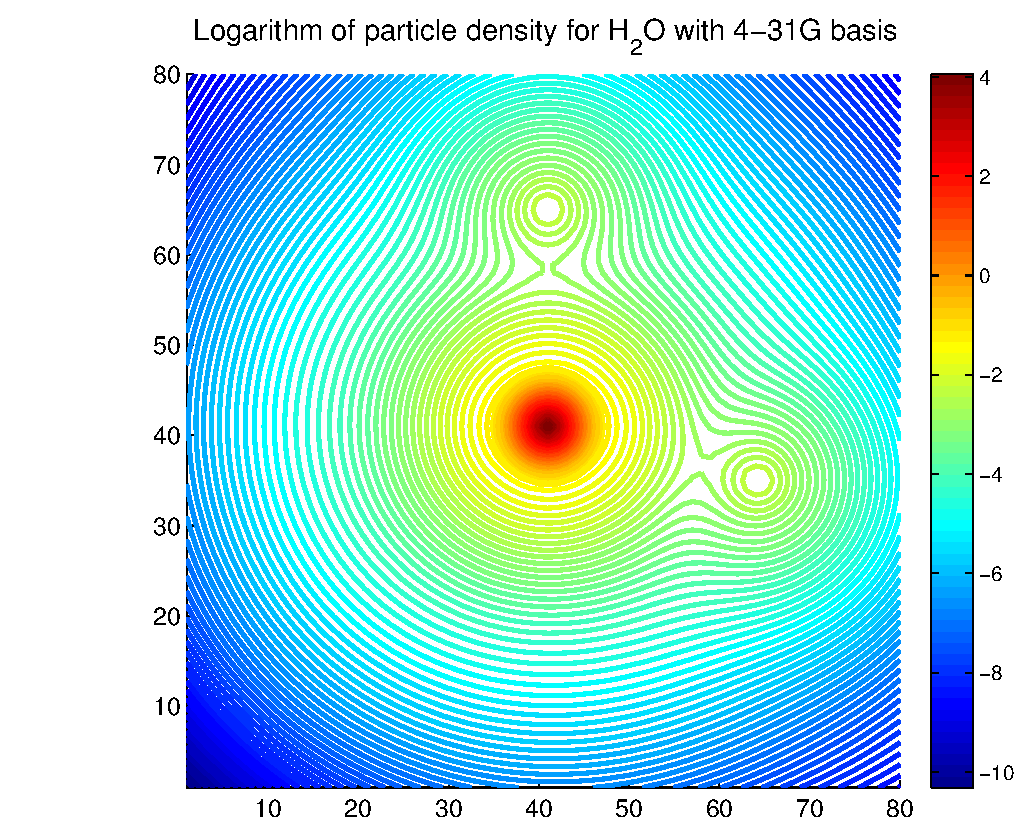
\includegraphics[width=0.45\textwidth]{./figures/H2Odensity_431g.pdf}
\caption{Electron density for H$_2$O with 4-31G basis functions on all atoms}
\end{figure}

\begin{figure}[h!tb]
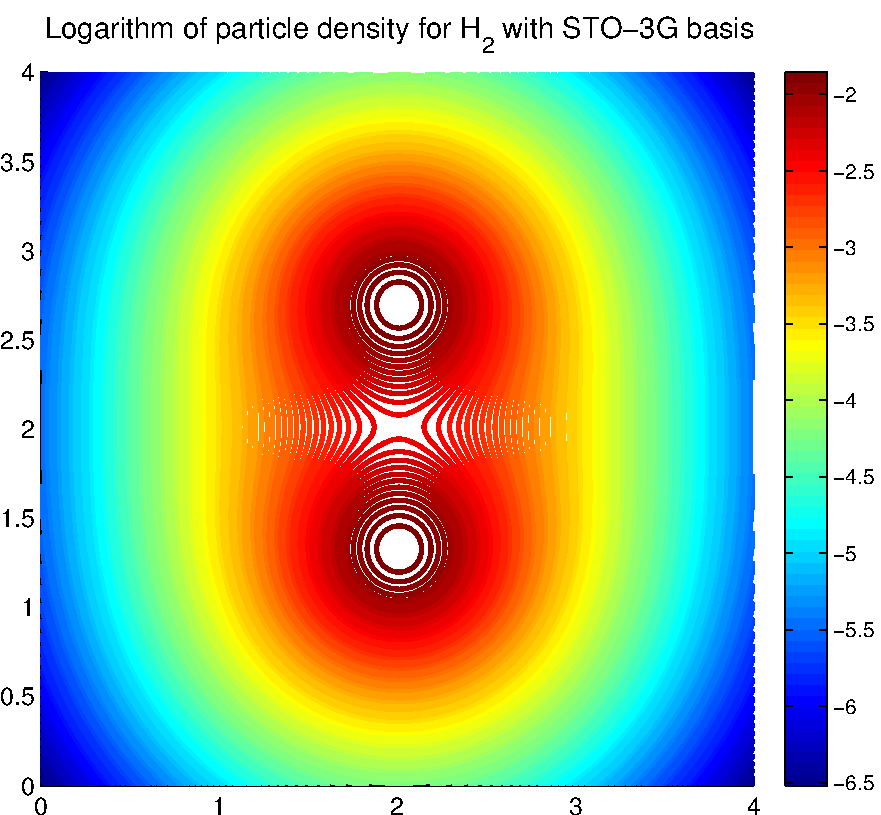
\includegraphics[width=0.45\textwidth]{./figures/H2density_sto3g.pdf}
\caption{Electron density for H$_2$ with STO3G basis functions on all atoms}
\end{figure}

\subsection{Implementation efficiency}
Almost all the time is spent calculating integrals over primitives. Therefore, it is valid to question whether one shold use contracted orbitals, and not just optimize coefficients for all the primitives. (This probla has some good expanation).



\begin{appendices}
\section{Terms}
\subsection{Unitary transformation}
A unitary transformation is a transformation that preserves the inner product of two vectors. A unitary matrix has the property $U^*U = I$. 

\end{appendices}


\bibliography{mendeleybib}
\end{document}
